\documentclass[10pt,twocolumn,letterpaper]{article}

\usepackage{cvpr}
\usepackage{times}
\usepackage{epsfig}
\usepackage{graphicx}
\usepackage{multirow}
\usepackage[table]{xcolor}
\usepackage{amsmath}
\usepackage[labelfont={bf,small},font=small]{caption}
\usepackage{amssymb}

\newcommand\crule[3][black]{\textcolor{#1}{\rule{#2}{#3}}}

% Include other packages here, before hyperref.

% If you comment hyperref and then uncomment it, you should delete
% egpaper.aux before re-running latex.  (Or just hit 'q' on the first latex
% run, let it finish, and you should be clear).
\usepackage[pagebackref=true,breaklinks=true,letterpaper=true,colorlinks,bookmarks=false]{hyperref}

% \cvprfinalcopy % *** Uncomment this line for the final submission

\def\cvprPaperID{****} % *** Enter the CVPR Paper ID here
\def\httilde{\mbox{\tt\raisebox{-.5ex}{\symbol{126}}}}

% Pages are numbered in submission mode, and unnumbered in camera-ready
\ifcvprfinal\pagestyle{empty}\fi
\begin{document}

%%%%%%%%% TITLE
\title{AGA : Attribute-Guided Augmentation}

\author{First Author\\
Institution1\\
Institution1 address\\
{\tt\small firstauthor@i1.org}
% For a paper whose authors are all at the same institution,
% omit the following lines up until the closing ``}''.
% Additional authors and addresses can be added with ``\and'',
% just like the second author.
% To save space, use either the email address or home page, not both
\and
Second Author\\
Institution2\\
First line of institution2 address\\
{\tt\small secondauthor@i2.org}
}

\maketitle
%\thispagestyle{empty}

%%%%%%%%% ABSTRACT
\begin{abstract}
We consider the problem of attributed-guided data augmentation, \ie,
the problem of synthesizing data such that an attribute of the synthesized 
data data is at a desired value or strength. This is specifically interesting
in scenarios where little data with no attribute annotation is 
is available for learning some task, but we have access to a large 
external corpus of heavily annotated samples. 
Specifically, we propose a deep encoder-decoder architecture, operating
in feature space, that facilitates to learn this mapping in 
an end-to-end manner. We demonstrate the utility of 
our architecture on the problem of one-shot object recognition.
As external data we leverage depth and pose information from the 
SUN RGB-D dataset and show that attribute-guided augmentation of
high-level CNN features substantially improves one-shot recognition over 
a couple of baselines.
\end{abstract}

%%%%%%%%% BODY TEXT
\section{Introduction}
\label{section:introduction}

Training deep neural networks in an end-to-end manner has
become the predominant strategy to approach difficult vision
problems, such as recognition \cite{Krizhevsky12a,Simonyan14a,He16a}, 
or detection \cite{Girshick15a, Ren15a}.
When training deep models, we benefit  
(1) from large amounts of training samples and (2) good coverage 
of the variability that we expect in previously unseen data. 
In scene recognition, for instance, we desire variability in the constellation and 
transient states of scene categories, whereas in object recognition, 
we desire variability in the specific incarnations of certain
objects, different lighting conditions, pose, or depth, just to 
name a few. Unfortunately, this variability is often dataset
specific and can cause substantial bias in recognition results 
\cite{Torralba11a}. To alleviate variability issues, at least to some 
extent, data augmentation techniques have become a popular 
and successful strategy, see, \eg, \cite{Krizhevsky12a, Chatfield14, Zeiler14a,
Charalambous16a,Hauberg16a,Rogez16a,Peng15a}. Aside from 
variability issues, augmentation obviously increase the amount of 
training data, which essentially allows to avoid overfitting and,
as a consequence, to obtain better models. 

\vskip0.5ex
While previously used augmentation techniques can be as simple as 
flipping, rotating, or extracting random crops from images, 
\emph{task-specific}, or \emph{guided} augmentation has 
the potential to lead to even better results on various tasks, see
Sec.~\ref{section:relatedwork}. Predominantly, augmentation
is typically done in input space, \ie, the space of images.
While this is not a particular problem with simple 
techniques, such as flipping, is can become computationally
expensive if more elaborate augmentation techniques are 
used. We argue that, in specific problems, augmentation might
as well be done in \emph{feature space}, especially in 
situations where features are input to subsequent learning
processes. This is common, \eg, in recognition problems, where
the softmax output of trained CNNs is often not used directly, but
activations at earlier layers are input to an additional 
discriminant classifer. The drawback of such approaches, 
however, is that augmentation requires \emph{guidance}, \eg,
in the form of external training data from which specific
augmentation models can be learned and then applied.

\begin{figure}[t!]
\centering{
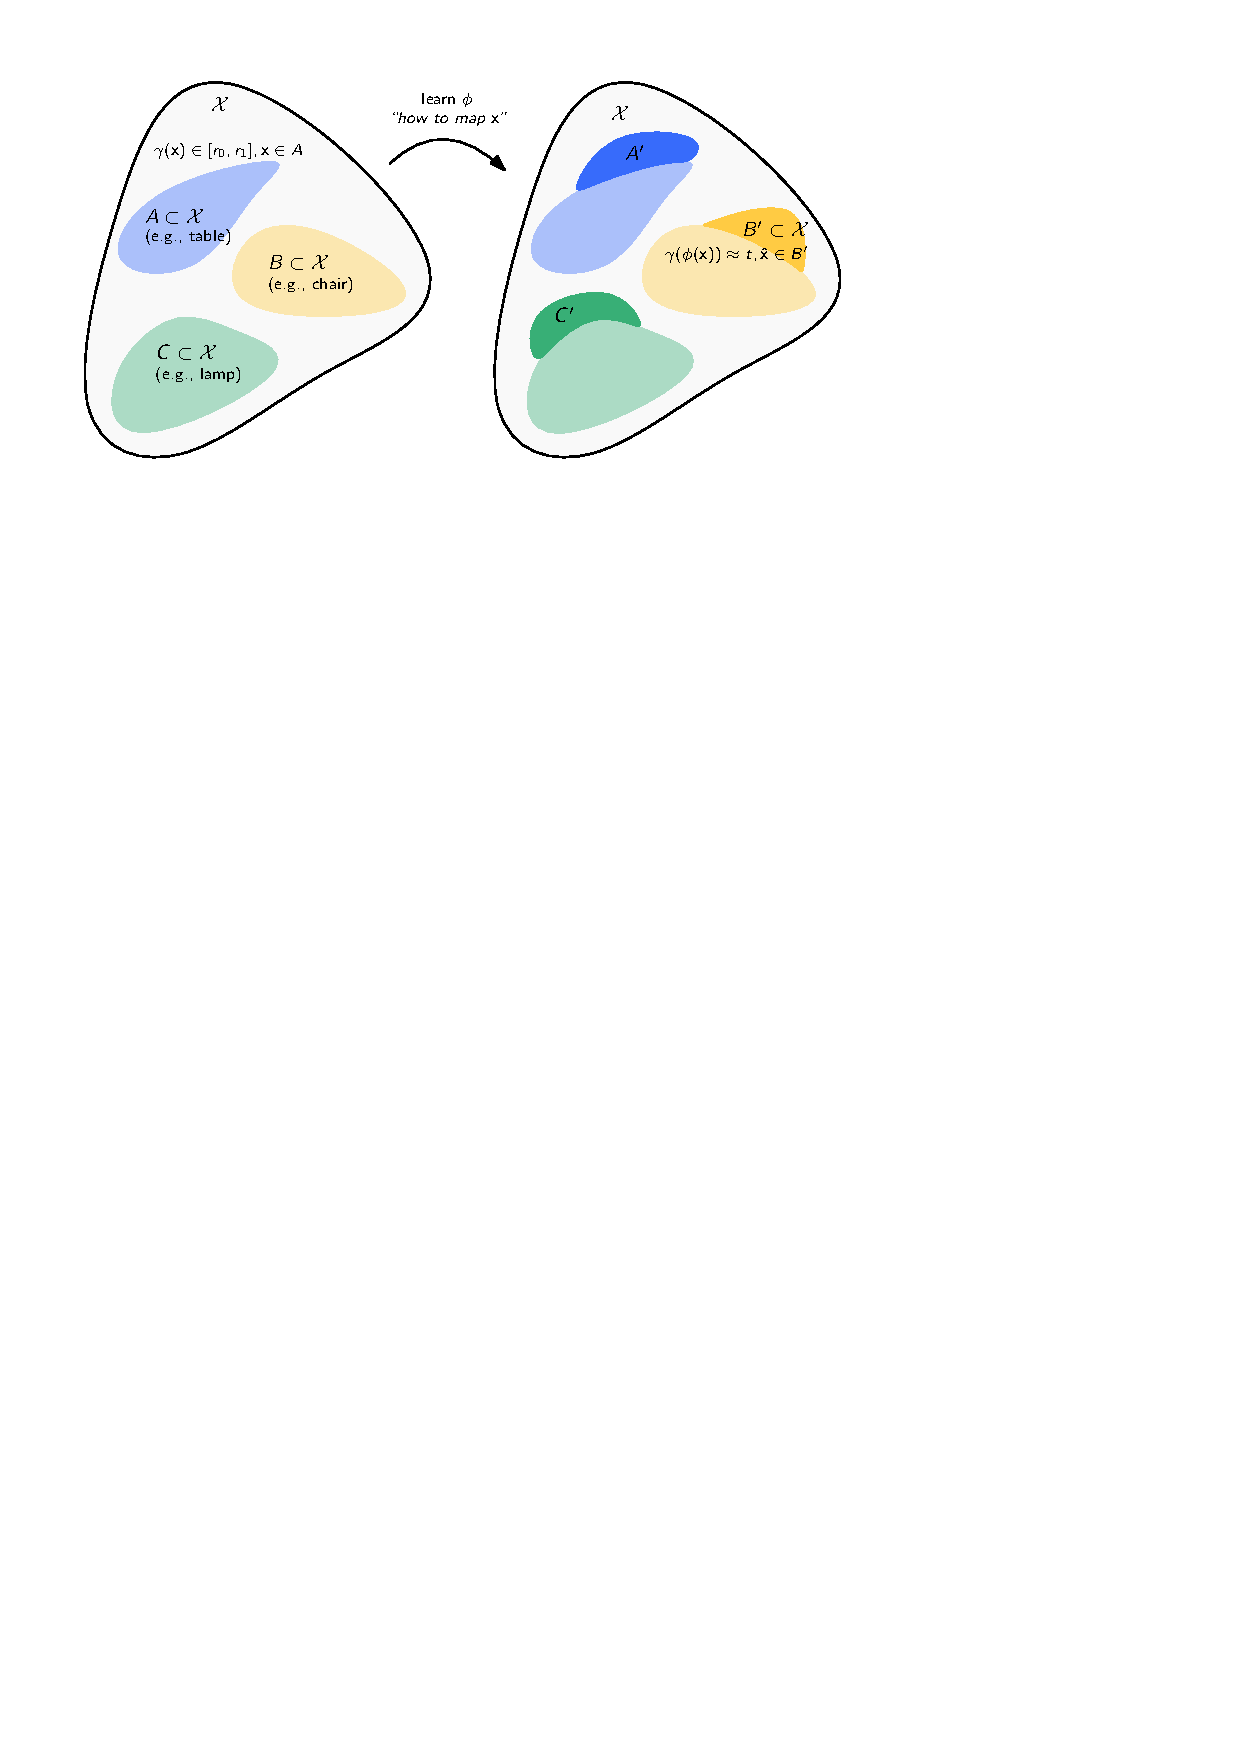
\includegraphics[width=0.99\columnwidth]{figures/Intro}
}
\caption{\label{fig:intro}Given an attribute
strength regressor $\gamma$, learn how to map a feature
$\mathbf{x} \in \mathcal{X}$, extracted from objects (\eg, chairs, tables)
with attribute strength in $[r_0,r_1]$, to a synthesized feature
$\mathbf{\hat{x} \in \mathcal{X}}$ such that (1) its predicted attribute
strength is close to the desired target attribute strenght 
$t$ and (2) the synthesized feature is ``close'' to $\mathbf{x}$; the latter
is required so that the \emph{object identity} can be
preserved.}
%Colored areas on the \emph{left} illustrate the partition
%of $\mathcal{X}$ for each object, whereas colored areas on the
%\emph{right} show the extended partition of $\mathcal{X}$ covered
%by synthesized features.}
\end{figure}

\vskip1ex
\noindent
\textbf{Contribution.} 
In this work, we propose such an augmentation technique
that learns to synthesize features, guided by desired values
for a set of auxiliary attributes, such as depth or pose.
We exemplify this technique in the context
of object recognition with few examples, one-shot recognition
in particular. Our objective is to leverage a large
\emph{external} database of images with attributes and learn how features
react to changes in those attributes; Fig.~\ref{fig:intro} illustrates
this concept. Intuitively, we aim for a greater coverage of the
feature space, induced by attribute variations.
In particular, our model(s) are trained in manner that 
is agnostic to the specific type of object. In other words, 
we learn a generic mapping function that captures the 
\emph{essence} of a change in the attribute values. 
Once these models
are trained, we can \emph{transfer} them to new, previously
unseen features of objects and perform synthesis with desired 
attribute values or strengths. We study the specific building
blocks of this approach in detail and eventually demonstrate
that guided augmentation in feature space improves 
recognition performance in a one-shot learning setting 
on previously unseen objects.

\vskip1ex
\noindent
\textbf{Organization.} Sec.~\ref{section:relatedwork} reviews
related work on data augmentation. 
Sec.~\ref{section:architecture} then introduces
the proposed encoder-decoder architecture for attribute-guided 
augmentation. In Sec.~\ref{section:experiments}, we evaluate each
part of the architecture and show experiments on one-shot object
recognition. Sec.~\ref{section:discussion} concludes the paper with
a discussion and an outlook on potential future directions.

\section{Related work}
\label{section:relatedwork}

Our review of related work primarily focuses on 
\emph{data augmentation} strategies. While many techniques
have been proposed in the context of training deep 
neural networks to avoid overfitting and increase variability
in the data, other (sometimes closely related) 
techniques have previously appeared in the context
of one-shot and transfer learning. We can roughly
group existing techniques into (1) 
\emph{generic} and computationally cheap 
approaches and (2) task-specific, or guided approaches
that are typically more computationally involved.

\vskip0.5ex
As a representative of the first category, Krizhevsky \etal \cite{Krizhevsky12a} 
leverage a set of label-preserving transformations, such 
as patch extraction + reflections, and PCA-based intensity
transformations, to increase training sample size. Similar techniques
are used by Zeiler and Fergus \cite{Zeiler14a}. In \cite{Chatfield14},
Chatfield and Zisserman demonstrate that
the augmentation techniques of \cite{Krizhevsky12a}
are not only beneficial for training deep architectures, but 
shallow learning approaches equally benefit from
such \emph{simple} and \emph{generic} schemes.

\vskip0.5ex
In the second category of guided augmentation techniques,
many approaches have recently been proposed.
In \cite{Charalambous16a}, \eg, Charalambous and Bharath
employ guided data augmentation in the context of
gait recognition. The authors suggest to simulate synthetic
gait video data (from avatars) over various confounding 
factors (such as clothing, hair, etc.) to extend the training corpus 
for deep gait recognition. Similar in spirit, Rogez and 
Schmid \cite{Rogez16a} recently proposed an image-based
synthesis engine for augmenting existing 2D human pose
data by photorealistic images with greater pose variability.
This is done by leveraging 3D motion capture (MoCap) data. 
3D data, in the form of synthetic CAD models, is also used
by Peng \etal \cite{Peng15a} to render synthetic images 
of objects (with varying pose, texture, background) that are then 
used to train CNNs for object detection. It is shown that
synthetic data is beneficial, especially in situations where few
(or no) training instances are available, but 3D CAD models
are. Su \etal \cite{Su15a} follow a similar pipeline
of rendering images from 3D models for 3D viewpoint 
estimation, however, with substantially more synthetic data
obtained, \eg, by additionally deforming existing 3D models
before rendering.

Another (data-driven) guided augmentation technique is 
introduced  by Hauberg \etal \cite{Hauberg16a}. The authors 
propose to \emph{learn} class-specific transformations on external 
training data, instead of manually specifying transformations
as in \cite{Krizhevsky12a,Zeiler14a,Chatfield14}. The learned
transformations are then applied to the samples of 
each class. Specifically, diffeomorphisms are learned
from data and encouraging results are demonstrated in the 
context of digit recognition on MNIST. Notably, this 
strategy is conceptually similar to earlier work by 
Miller \etal \cite{Miller00a} on one-shot learning, where 
the authors synthesize additional data for digit images 
via an iterative process, called \emph{congealing}. During 
that process, external images of a given category are aligned by
optimizing over a class of geometric transforms (\eg, 
affine transforms). These transformations are then applied
to single instances of the new categories to increase 
data for one-shot learning.

\vskip1ex
Marginally related to our work, we remark that alternative 
approaches to implicitly learn spatial transformations have
been proposed. For instance, Jaderberg \etal \cite{Jaderberg15a}  
introduce \emph{spatial transformer} modules that can be
injected into existing deep architectures to implicitly capture 
spatial transformations inherent in the data, thereby improving
invariance to this class of transformations.

\vskip1ex
While \emph{all} previously discussed methods essentially aim to 
\emph{augment the input space} (\ie, the space of images) for 
training CNNs, our approach is different in that we aim for
\emph{augmentation in feature space}. Along these lines, the 
approach of Kwitt \etal \cite{Kwitt16a} conceptually 
similar to our work. In particular, the authors suggest to learn
how features change as a function of the strength of certain 
transient attributes (such as sunny, cloudy, or foggy) in 
a scene-recognition context. These models are 
then transfered to previously unseen data for one-shot recognition.
However, different to our approach, the learned models 
are simple linear regressors and learning is done in a 
\emph{scene-category specific} manner.
Contrary to that, in our work, we learn deep non-linear
models in a \emph{category-agnostic} manner which 
enables straightforward application to object recognition 
in a transfer-learning setup.

\section{Architecture}
\label{section:architecture}

\noindent
\textbf{Notation.}
To describe our architecture, we let $\mathcal{X}$ denote 
our feature space, $\mathbf{x} \in \mathcal{X}$ denotes a
feature vector (\ie, a representation of an object) 
and $s \in \mathbb{R}_+$ denotes the strength 
of a specific attribute $A \in \mathcal{A}$ associated with $\mathbf{x}$. We
assume that this attribute can be reasonably binned into intervals
$[l_i,h_i]$, where $l_i,h_i$ denote the lower and upper bounds of the $i$-th interval. We let $T$ denote the number of such intervals.

\vskip1ex
\noindent
\textbf{Objective.}
On a conceptual level, we aim for a mapping function $\phi$ which,
given a desired covariate strength $t$ for a specific attribute $A$, 
transforms input features such that the attribute strength changes
in a controlled manner to a desired target value. More formally, we aim to learn
\begin{equation}
\phi: \mathcal{X} \times \mathbb{R}_+ \rightarrow 
\mathcal{X}, (\mathbf{x},t)\mapsto \hat{\mathbf{x}}, \quad \text{s.t.}\quad 
\gamma(\hat{\mathbf{x}}) \approx t\enspace. 
\label{eqn:general}
\end{equation}
Since, the formulation in Eq.~\eqref{eqn:general} 
is overly generic, we constrain the 
problem to the case where we aim to learn different
$\phi_i^k$ for a selection of intervals $[l_i,h_i]$ and a selection
of $K$ given covariate targets $t_k$. While
this simplifies the problem, it requires a 
good \emph{covariate predictor}, since, 
otherwise, we could not decide with $\phi_i$ to use. 
During testing, we (1) predict the covariate strength, \ie, 
$\gamma(\mathbf{x}) =
\hat{t}$, and then (2) synthesize features as
$\hat{\mathbf{x}}_i = 
\phi_i(\mathbf{x})$ for $i=1,\ldots,T$ if $\hat{t} 
\in [l_i,h_i]$. Next, we discuss each 
component of this architecture in detail.

\subsection{Covariate regression}
\label{subsection:covariateregression}

An essential part of our architecture is the covariate
regressor $\gamma: \mathcal{X} \rightarrow \mathbb{R}_+$ 
for a given attribute $A$. This covariate regressor 
takes as input a feature $\mathbf{x}$ and predicts its
strength, \ie, $\gamma(\mathbf{x}) = \hat{t}$. While
$\gamma$ could, in principle, be implemented by 
a variety of approaches, such as support vector regression
or Gaussian processes, we use a two-layer neural network
instead, to accomplish this task. This is not an arbitrary 
choice, as it will later enable us to re-use this building 
block in the learning stage of the feature regressor.
The architecture of the covariate regressor is shown in 
Fig.~\ref{fig:COR}, consisting of two linear layers, 
interleaved by batch normalization and ReLU 
activations.

\begin{figure}[h!]
\centering{
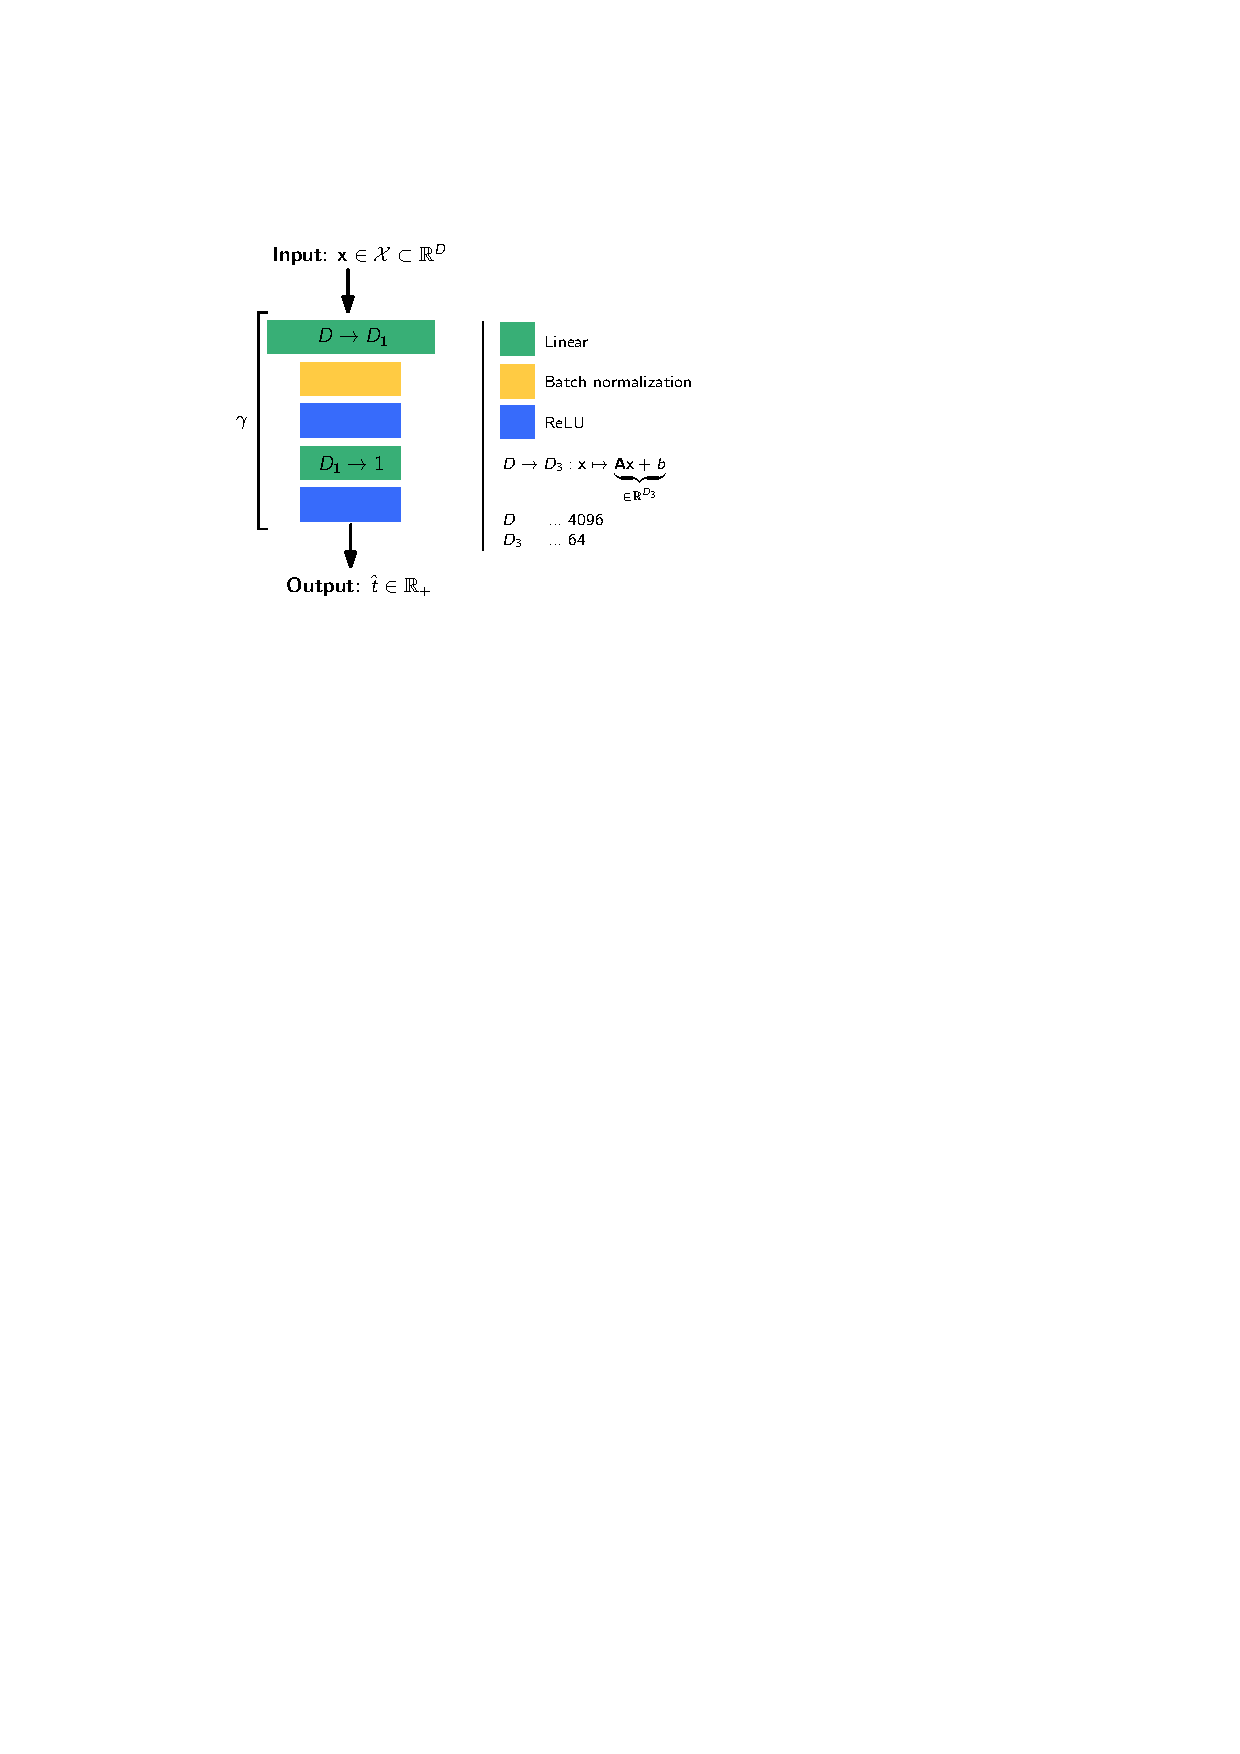
\includegraphics[scale=0.8]{figures/COR}}
\caption{Architecture of the covariate regressor.\label{fig:COR}}
\end{figure}

\vskip0.5ex
\noindent
\textbf{Learning.} The covariate regressor can easily
be trained from a collection of $N$ training tuples $
\{(\mathbf{x}_i,s_i)\}_{i=1}^N$. We remark that for 
this part of the architecture, we do not need any binning 
of the covariate.

\subsection{Feature regression}
\label{subsection:aug}

To implement $\phi$, we design an encoder-decoder
architecture, reminiscent of a conventional autoencoder.
Our objective, however, is not encode and then reconstruct 
the input, but to produce an output that resembles a feature 
of an object at a specific covariate strength.

In other words, the \emph{encoder} essentially learns to extract
the essence of features; the \emph{decoder}
then takes the encoding result and decodes it to the desired result. In
its simplest form, we can formulate the optimization problem as
\begin{equation}
\min_{\phi \in \mathcal{C}} L(\mathbf{x},t,\phi) = (\gamma(\phi(\mathbf{x}))-t)^2\enspace,
\label{eqn:unconstrained}
\end{equation}
where the minimization is 
over a suitable class of functions $\mathcal{C}$. Notably, when implementing 
$\phi$ as an encoder-decoder network with loss 
$(\gamma(\phi(\mathbf{x}))-t)^2$, we have little control over the decoding 
results in the sense that we cannot guarantee that the \emph{identity}
of the input is preserved. In other words, features from a particular class
of objects might map to features that are no longer recognizable as
this class, as the encoder-decoder will \emph{only} learn to ``fool'' the 
covariate regressor $\gamma$.
For that reason, we add a \emph{regularizer} to the objective
of Eq.~\eqref{eqn:unconstrained}, \ie, we require that the 
decoding result needs to be close, \eg, in the $L_2$ norm, to the
input. This changes the optimization problem to
\begin{equation}
\min_{\phi \in \mathcal{C}} L(\mathbf{x},t,\phi) = \underbrace{(\gamma(\phi(\mathbf{x}))-t)^2}_\text{Target mismatch} + 
\lambda \underbrace{\| \phi(\mathbf{x}) - \mathbf{x} \|^2}_{\text{Regularizer}}
\enspace.
\label{eqn:constrained}
\end{equation}
Interpreted differently, this resembles the loss of an autoencoder network with an added \emph{target mismatch} term. The encoder-decoder network that implements the function class $\mathcal{C}$ 
to learn $\phi$ is shown Fig.~\ref{fig:EDN}. 
The core building block is a combination of a linear layer, 
batch normalization, ELU \cite{Clevert16a}, followed by dropout 
\cite{Srivastava14a}. After the final linear
layer, we add one ReLU layer to enforce $\mathbf{x} \in \mathbb{R}^D_+$.

\begin{figure}
\centering{
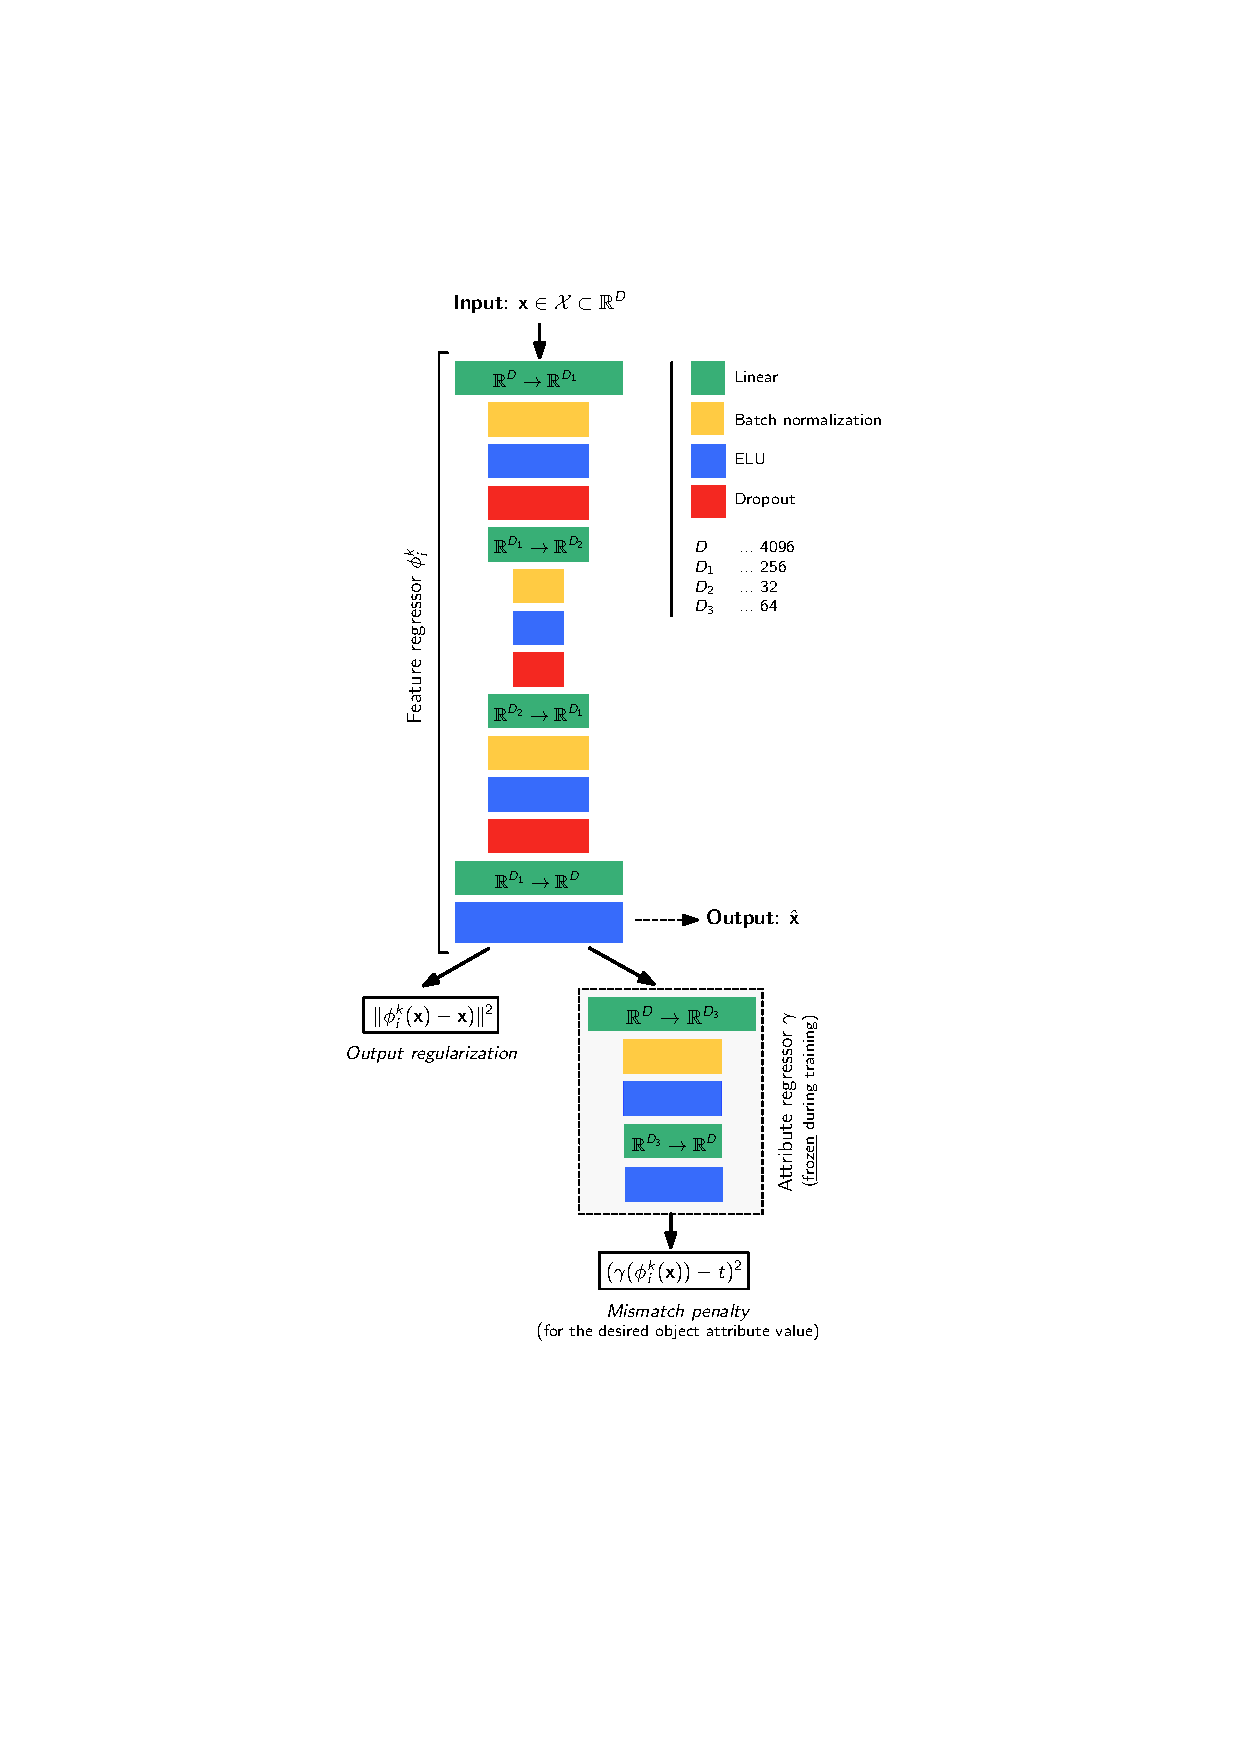
\includegraphics[scale=0.80]{figures/EDN}}
\caption{Illustration of the proposed encoder-decoder network.
During \emph{training}, the covariate regressor is appended to
the network, whereas, for \emph{testing} this part is removed.
\label{fig:EDN}}
\end{figure}

\vskip0.5ex
\noindent
\textbf{Learning.} Learning the encoder-decoder network of Fig.~\ref{fig:EDN}
first requires an already trained covariate regressor $\gamma$ for an attribute
$A \in \mathcal{A}$. During training, this covariate
regressor is appended to the network and its weights are frozen.
Hence, only the encoder-decoder weights
are updated. To train one $\phi_i^k$ for each interval $[l_i,h_i]$ and
target covariate strength $t_k$, we partition
the training data into subsets $\mathcal{S}_i$, such that
$\forall (\mathbf{x}_n,s_n) \in \mathcal{S}_i: s_n \in [l_i,h_i]$. Each
$\phi_i^k$ is then trained using only those data tuples. We
note that, since training is done in feature space, we have no 
convolutional layers and consequently training is computationally
cheap. For testing, the covariate regressor is removed and only 
the trained encoder-decoder network is used.

\section{Experiments}
\label{section:experiments}

In our experiments, we first discuss generation of training data, 
then evaluate every part of our architecture separately and eventually
demonstrate its utility on the problem of one-shot object recognition
in a transfer learning setting.

\vskip1ex
\noindent
\textbf{Dataset.} We use the SUN {RGB-D} dataset from 
Song \etal \cite{Song15a}. This dataset contains 10335 
RGB images with depth information, as well as detailed 
annotations for more than 1000 objects in the form of 
2D and 3D bounding boxes.
In our setup, we will use depth and pose information of
objects as our attributes, \ie, $\mathcal{A} = \{\texttt{Depth}, 
\texttt{Pose}\}$. For each ground-truth 2D bounding box 
of an object, we use the depth value at its centroid. Pose
information is computed from the 3D bounding box of 
each object. In all experiments, we use the first
5335 images as our \emph{external database}, \ie, the database
for which we assume availability of attribute annotations.
The remaining 5000 images are used for testing; more details
are given in the specific experiments.

\vskip1ex
\noindent
\textbf{Training data.} Notably, in SUN RGB-D, the
number of instances of each object class are not 
evenly distributed. This is simply because this dataset
was not designed for object recognition. Consequently,
images are also not object-centric, meaning that there
is substantial variation in the location of objects and 
the depth and pose at which they occur. This makes
it difficult to extract a sufficient and balanced number
of features in case we would use the ground-truth 
bounding boxes. We circumvent this problem, by
leverage the Fast-RCNN detector of \cite{Girshick15a} 
with object proposals, generated by selective search 
\cite{Uijlings13a}. Specifically, we finetune the ImageNet 
model used in \cite{Girshick15a} to SUN RGB-D, using
the same 19 objects as in \cite{Song15a}. We then run 
the detector on the \emph{training data} and keep 
bounding boxes with detection scores $>0.5$. 
The associated R-CNN activations (at the \texttt{FC7} layer) 
are then used as our features $\mathbf{x}$.
As this strategy generates a larger number of features 
(compared to the number of ground-truth bounding
boxes), we can balance the training data in the sense
that we can select an equal number of activations per object
for training (1) the covariate regressor and (2) the 
encoder-decoder network.

\vskip1ex
\noindent
\textbf{Implementation.} The covariate regressor and 
encoder-decoder network are implemented in \texttt{Torch}.
All models are trained using \texttt{Adam} \cite{Kingma15a}. 
For the covariate regressor, we train with a batch size of 300, 
30 epochs and a learning rate of 
$0.001$. The encoder-decoder network is trained with 
a batch size of 128, 30 epochs and the same learning 
rate. The dropout probability during training is set to $0.25$.
No dropout is used for testing. On a Linux system, running
Ubuntu 16.04, with 128 GB of memory and one NVIDIA 
Titan X, training one model (\ie, one $\phi_i^k$) takes 
$\approx 30$ seconds. The relatively low demand on 
computational resources highlights the advantage of 
augmentation in feature space, as no convolutional layers
need to be trained.

\subsection{Covariate regression}
\label{subsection:EvalCovariateRegression}

In principle, we can identify two strategies to train and assess
regression performance for our attributes. \emph{First}, we could 
train \emph{object-specific} regressors 
$\gamma_k, k \in \{1,\ldots, |\mathcal{C}|\}$, \ie, one regressor
for each object category. This would, however, prevent us from 
using the regressor(s) in a transfer-learning setting, as we might not
have seen objects that appear in a target dataset during training. 
An alternative, \emph{second} 
strategy is to train \emph{object-agnostic} regressors 
using features from all objects together. We evaluate both 
strategies, in order assess the potential loss in prediction
performance in the object-agnostic setting. 
Table~\ref{table:maeCOR} lists
the median-absolute-error (MAE) per object, evaluated for 
19 object categories extracted from images in 
the testing portion of SUN RGB-D. 
\begin{table}[t!]
\small
\centering{
\begin{tabular}{rcccc}
\hline
\multirow{ 2}{*}{\textbf{Object}} & \multicolumn{2}{c}{\textbf{Depth} (MAE [m])}  & \multicolumn{2}{c}{\textbf{Pose} (MAE [deg])}\\
& per-object & agnostic  & per-object & agnostic \\
\hline
 bathtub & 0.31 & 1.05 & 36.02 & 108.17\\ 
                 bed & 0.40 & 0.30 & 44.51 & 70.51\\ 
           bookshelf & 0.64 & 0.45 & 50.61 & 95.44 \\ 
                 box & 0.49 & 0.59 & 29.69 & 59.37\\ 
               chair & 0.40 & 0.31 & 37.82 & 53.08 \\ 
             counter & 0.51 & 1.45 & 43.81 & 13.47 \\ 
                desk & 0.39 & 0.36& 48.24 & 47.07 \\ 
                door & 0.41 & 2.03 & 45.62 & 51.84\\ 
             dresser & 0.27 & 0.44 & 65.42 & 63.82\\ 
         garbage bin & 0.34 & 0.32 & 45.93 & 54.43\\ 
                lamp & 0.40 & 1.04 & 30.51 & 132.49\\ 
             monitor & 0.27 & 0.26 & 28.90 & 69.48\\ 
         night stand & 0.53 & 0.85& 28.19 & 99.40 \\ 
              pillow & 0.39 & 0.46 & 34.93 & 73.19\\ 
                sink & 0.17 & 0.20& 60.04 & 59.43 \\ 
                sofa & 0.41 & 0.33& 32.25 & 51.51  \\ 
               table & 0.39 & 0.30 & 41.52 & 50.60\\ 
                  tv & 0.47 & 0.75& 32.33 & 61.77  \\ 
              toilet & 0.24 & 0.23 & 21.58 & 50.89\\ 
		\hline
              \end{tabular}}
\caption{\label{table:maeCOR} Median-Absolute-Error (MAE), for depth / pose, 
of the covariate regressor, evaluated on \emph{19 objects} from \cite{Song15a}.
In our setup, the pose estimation error quantifies the error in predicting a
rotation around the $z$-axis.}
\end{table}
As we can see, training in an object-specific manner leads
to a lower MAE for most objects, both for depth and pose. 
This is not surprising, since the training data is more specialized
to each particular object, which essentially amounts to solving
simpler sub-problems. In many cases, especially for depth, 
the object-agnostic regressor performs on par, except for 
object classes with very few samples (\ie, lamp, door, etc.). 
We remark that, in general, pose estimation from 2D data is
a substantially harder problem then depth estimation.


\subsection{Feature regression}
\label{subsection:EvalFeatureRegression}

In this section, we assess the performance of the feature regressor 
$\phi_i^k$, \ie, the part of our architecture that is used to generate 
synthetic features.

In all experiments, we use an overlapping sliding window to
generate the intervals $[l_i,h_i]$ for a specific attribute. In case
of \emph{depth}, we set $[l_0,h_0] = [0,1]$ and shift by $0.5$ meter
to cover the full range of the attribute in the training data. For
augmentation, we use target depth values of $0.5, 1, \ldots, \max(A)$.

\emph{First}, to assess the performance of $\hat{\mathbf{x}} = \phi_i^k(\mathbf{x})$
on the task of actually synthesizing features such that $\gamma(\hat{\mathbf{x}}) \approx t$. 
Table~\ref{table:ednnonseen} lists the MAE per object, \ie, $|\gamma(\hat{\mathbf{x}}) -t|$, 
averaged over all target values. \emph{Second}, we assess how much 
the original features $\mathbf{x}$ differ from their synthesized variants
$\phi_i^k(\mathbf{x})$. Since, $\|\phi_i^k(\mathbf{x})-\mathbf{x}\|^2$ is 
hard to interpret, we compute the Pearson correlation coefficient $\rho$ of each original
feature and its synthesized versions instead,\ie, $\rho(\mathbf{x},\phi_i^k(\mathbf{x}))$.
 Results are reported in Table~\ref{table:ednnonseen}.
\begin{table}[t!]
\small
\centering{
\begin{tabular}{r|cc}
\hline
\textbf{Object} & $\rho$ & \textbf{Depth} (MAE [m])\\
\hline
picture 		& 0.66 $\pm$ 0.08 & 0.13 $\pm$ 0.12 \\ 
ottoman 		& 0.69 $\pm$ 0.08 & 0.13 $\pm$ 0.11 \\ 
whiteboard 	& 0.66 $\pm$ 0.06 & 0.16 $\pm$ 0.14 \\ 
fridge 		& 0.68 $\pm$ 0.08 & 0.13 $\pm$ 0.11 \\ 
counter 		& 0.75 $\pm$ 0.07 & 0.10 $\pm$ 0.09 \\ 
books 		& 0.73 $\pm$ 0.07 & 0.11 $\pm$ 0.10 \\ 
stove 		& 0.70 $\pm$ 0.07 & 0.11 $\pm$ 0.10 \\ 
cabinet 		& 0.73 $\pm$ 0.08 & 0.11 $\pm$ 0.10 \\ 
printer 		& 0.72 $\pm$ 0.07 & 0.11 $\pm$ 0.11 \\ 
computer 		& 0.82 $\pm$ 0.09 & 0.09 $\pm$ 0.09 \\ 
\hline
\end{tabular}}
\caption{\label{table:ednnonseen}Quality assessment of $\phi(\mathbf{x})$ on a 
selection of 10 \emph{unseen objects}: for each object, 
$\rho$ lists the average Pearson correlation of all original features
from that object with respect to the corresponding synthesized features. 
The \emph{depth} column lists the average MAE of 
the predicted attribute value with respect to the desired target 
values.}
\end{table}
As we can see, the correlation is high, indicating high similarity
of synthesized features $\hat{\mathbf{x}}$ with respect to their 
original versions. Further, the MAE is low, indicating that 
$\phi_i^k$ can transform features such that the covariate predictor
outputs the desired target value.

\subsection{One-shot object recognition}
\label{subsection:one-shot}

Finally, we demonstrate the utility of our approach on
the problem of one-shot object recognition in a transfer
learning setup. Specifically, we aim to learn attribute-guided 
augmenters from instances of object categories in an 
external database. We denote this collection of object 
categories as our \emph{source categories} $\mathcal{S}$. 
Given one instance from a collection of a completely different 
collection of object classes, denoted as the \emph{target classes} 
$\mathcal{T}$, we aim to train a discriminant classifier 
$C$ on $\mathcal{T}$, \ie, $C: \mathcal{X} \rightarrow \{1,\ldots,|\mathcal{T}|\}$. 
Formally, in this setup  $\mathcal{S} \cap \mathcal{T} =
\emptyset$. This can be considered a variant of 
transfer learning, since we transfer knowledge from 
instances of $\mathcal{S}$ to instances of $\mathcal{T}$ 
\emph{and now knowledge about $\mathcal{T}$ is 
avaialble a-priori.} 

\vskip1ex
\noindent
\textbf{Setup.} To evaluate performance on one-shot object 
recognition for \emph{unseen} object categories, we adhere
to the following setup. First, we  randomly select two collections
of 10 object categories with more than 100 ground truth bounding 
boxes from SUN RGB-D. These object categories constitute our 
set of target classes $\mathcal{T}_1$\footnote{$\mathcal{T}_1$ = \{picture, whiteboard, fridge, counter, books, stove, cabinet, printer, computer, ottoman\}}
 and $\mathcal{T}_2$\footnote{$\mathcal{T}_2$ = \{ mug, telephone,bowl, bottle,scanner, microwave, coffee table, recycle bin, cart, bench\}}. 
 We
also construct a third set of target classes 
$\mathcal{T} = \mathcal{T}_1 \cup \mathcal{T}_2$ and remark that  $\mathcal{T}_1
\cap \mathcal{T}_2 = \emptyset$. Consequently, we have two
10-class problems and one 20-class problem.
For each object category in the target classes, we then 
collect RCNN 
\texttt{FC7} features from SUN RGB-D images that were left-out 
as the testing set. This guarantees (1) that we have never seen
the image, nor (2) the object category during training.

We also note that our goal here is \emph{not}
to jointly detect and recognize objects, but simply to demonstrate
the utility of our augmentation technique on the task of 
distinguishing previously unseen objects from just one sample.
As a \emph{baseline}, we train a linear C-SVM using only the
single instances of each object category. We use exactly the
same parameter settings of the linear SVM, but then train on
the single instances + features synthesized by our approach.
These experiments are repeated 500 times and the average 
recognition accuracy is reported. Table XXX lists the results.





\noindent
\textbf{Remark.} Notably, the design of this experiment is somewhat 
similar to \cite[Section 4.3.]{Peng15a}, with the exception 
that we (1) \emph{do not} detect objects, (2) augmentation
is performed in feature space and (3) no 
object-specific information is available. The latter is 
important, since \cite{Peng15a} assumes the existence of 
3D CAD models for objects in $\mathcal{T}$ from which 
synthetic images are generated.

\vskip1ex
\noindent
\textbf{Results.} Table XXX reports classification accuracy 

\begin{table}
\begin{tabular}{r|ccccc}
& \textbf{Baseline} &  \textbf{Ours} (\textbf{D}) & \textbf{Ours} (\textbf{P}) & \textbf{Ours} (\textbf{D+P}) \\
\hline
$\mathcal{T}_1$  & 34.95  & 38.58 & & \\
$\mathcal{T}_1$ & 24.27  & 28.30 & & \\
$\mathcal{T}_2$  & 23.34  & 25.80 & & \\
\hline
\end{tabular}
\end{table}





\section{Discussion}
\label{section:discussion}



{\small
\bibliographystyle{ieee}
\bibliography{egbib,halucination}
}

\end{document}
